\section{LLM-Controlled Agent}
\label{sec:llm}

The LLM-controlled agent (Agent B) uses a local Large Language Model to transform
natural-language requests into structured Deliveroo.js actions. It combines an autonomous
fallback policy with an interactive chat interface: when no request is pending the agent behaves
autonomously; when a user message arrives, the LLM temporarily takes responsibility for
high-level planning. The LLM never receives unrestricted control: it returns a strict JSON
object containing a textual response and a plan composed only of supported tools, conditions,
and bounded loops, which the local application parses and executes.

\subsection{Architecture and execution flow}
The main component, \texttt{LlmAgent.js}, manages the Deliveroo.js connection, local world
state (\texttt{WorldModel.js}: map, agent position, visible parcels, delivery and spawning
tiles), autonomous behaviour, user requests, and LLM plan execution. When a chat request is
received: the request is queued; the agent enters \texttt{LLM\_MODE}, pausing autonomous
decisions (avoiding the autonomous policy and the LLM plan steering the agent toward different
targets); \texttt{promptBuilder.js} combines the user message, a compact world snapshot, and
persistent memory (\texttt{memory.txt}, storing learned facts, reward observations, and
strategy rules); \texttt{ollama.js} queries a local Ollama model; \texttt{parser.js} interprets
and executes the returned plan; finally the agent resumes its fallback policy. A guard prevents
concurrent request processing. Figure~\ref{fig:llm-pipeline} summarises this pipeline.

\begin{figure}[htbp]
    \centering
    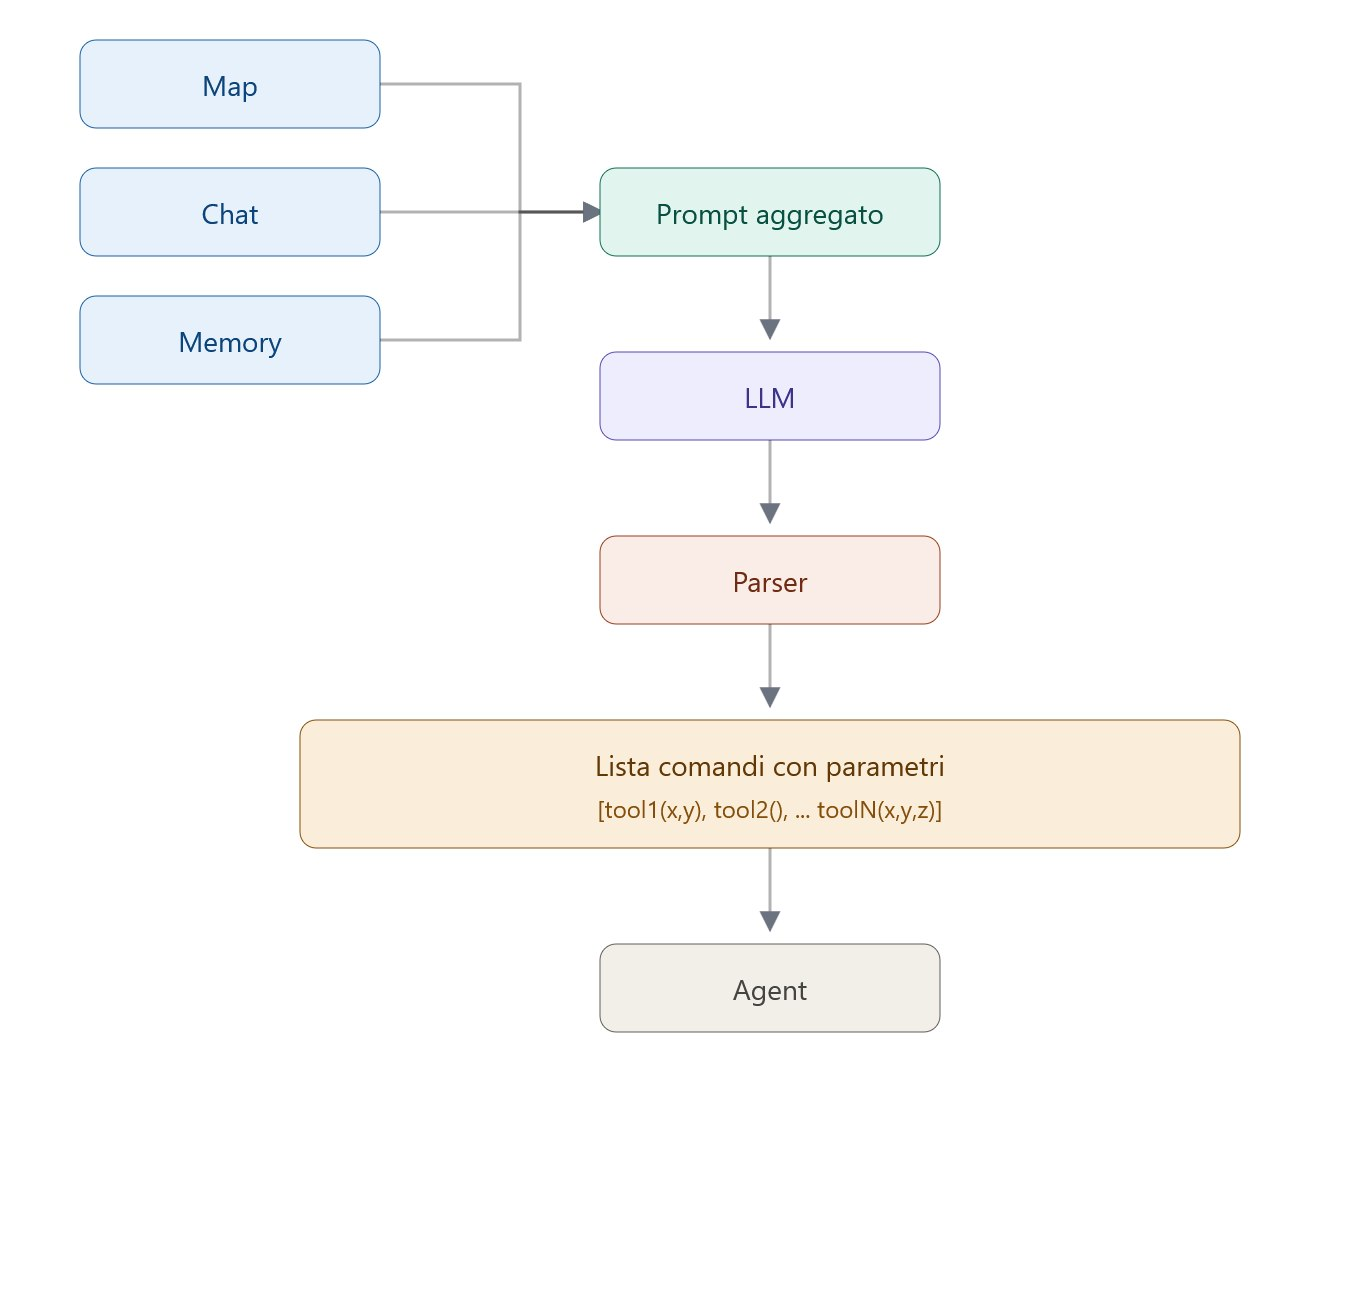
\includegraphics[width=0.56\linewidth, trim={50 250 90 20}, clip]{figures/llm_pipeline.jpg}
    \caption{LLM-controlled agent pipeline. The map state, chat request, and persistent memory
    are aggregated into a single prompt; the LLM output is parsed into a parameterised command
    list (\texttt{tool$_1$(x,y)}, \dots, \texttt{tool$_N$(x,y,z)}), which is then executed by
    the agent.}
    \label{fig:llm-pipeline}
\end{figure}

Outside \texttt{LLM\_MODE}, the fallback strategy prioritises on-tile actions (pickup,
delivery), then targets: deliver when carrying many parcels, move toward the nearest reachable
free parcel, deliver when carrying with no visible parcel, otherwise explore. Navigation uses
A* with visible agents treated as temporary obstacles, moving one step at a time so the world
state refreshes between movements.

\subsection{Constrained plan interpreter and tools}
The LLM must return JSON only, with a \texttt{chat} field shown to the user and a \texttt{plan}
field: a small domain-specific language of direct tool calls,
\texttt{if}/\texttt{then}/\texttt{else} branches, and condition-guarded \texttt{loop} blocks ---
never arbitrary code. Tool names resolve through a predefined mapping, so the LLM can invoke
only intentionally exposed functions: \texttt{move\_to} (A* navigation with step limits),
\texttt{pick\_up\_parcel} / \texttt{put\_down\_parcel}, \texttt{find\_and\_get\_a\_parcel} (a
reactive search that refreshes its target after each movement, handling parcels that expire or
are taken by rivals), \texttt{calculator}, \texttt{add\_to\_memory}, and
\texttt{reply\_to\_server}. The interpreter applies defensive limits --- bounded loop iterations,
abort after repeated failed iterations, termination on fatal movement or network errors ---
because generated plans may be incomplete or based on outdated observations.

\subsection{MCP-based control of a second agent}
The system can coordinate a separate agent (\texttt{BdiLlmTestAgent.js}) through the Model
Context Protocol: the second agent runs independently, connects to Deliveroo.js, and exposes
selected capabilities via an HTTP MCP endpoint. The LLM agent drives it through explicit typed
proxy tools (\texttt{agent\_move\_to}, \texttt{agent\_pick\_up\_parcel},
\texttt{agent\_put\_down\_parcel}, \texttt{agent\_find\_and\_get\_a\_parcel},
\texttt{agent\_get\_state}), refreshing its state before evaluating conditions that involve it.
This provides process separation: the LLM cannot touch the remote agent's internals, only a
restricted, typed action interface.

\subsection{Web interface}
The \texttt{webchat.js} component provides a browser chat panel with plan visualisation,
receiving messages over HTTP and streaming replies via Server-Sent Events.
Figure~\ref{fig:webchat-example} shows a request mixing an informational question with a
movement task; the LLM answers the question and emits four explicit \texttt{move\_to} actions.
More complex plans combine bounded local collection loops, delivery actions, and remote MCP
commands for the second agent.

\begin{figure}[htbp]
    \centering
    \begin{minipage}[c]{0.66\linewidth}
        \centering
        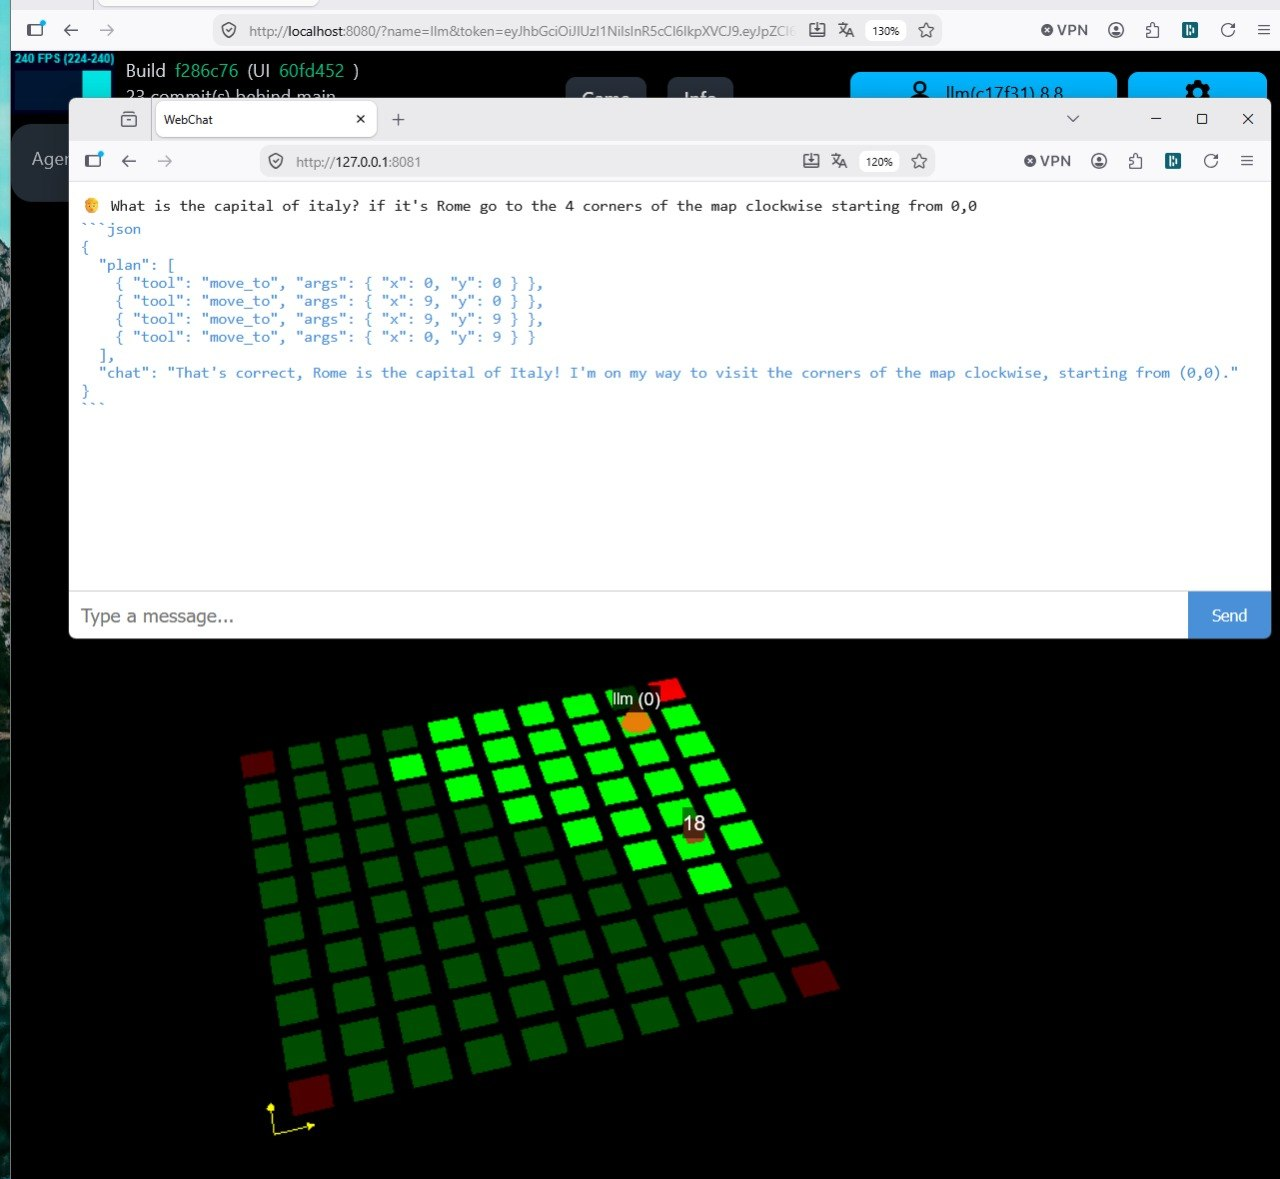
\includegraphics[width=\linewidth]{figures/webchat_example.jpg}
    \end{minipage}\hfill
    \begin{minipage}[c]{0.30\linewidth}
        \centering
        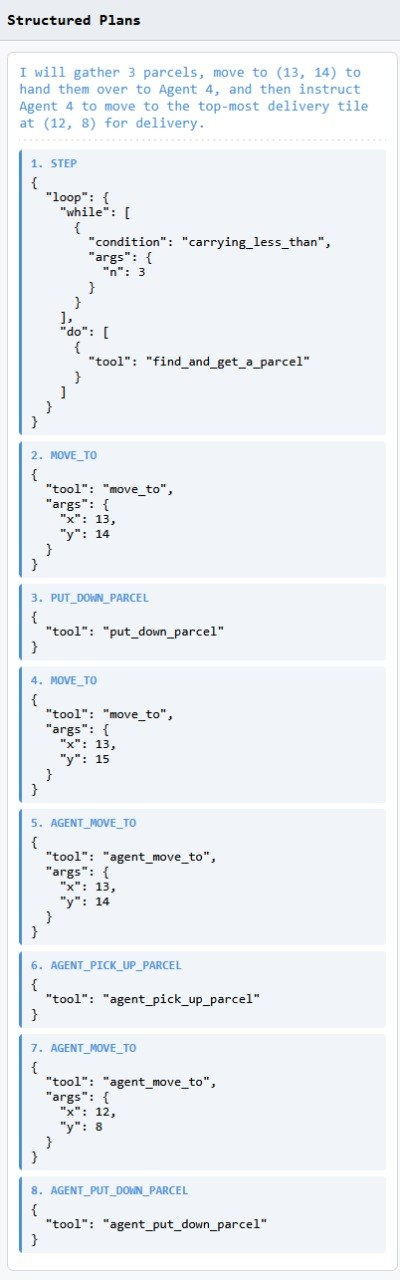
\includegraphics[height=7.8cm,keepaspectratio]{figures/complex_plan.jpg}
    \end{minipage}
    \caption{Left: web-chat example --- the agent answers a natural-language request and
    generates a JSON plan with four coordinate-based movement actions. Right: a multi-step plan
    combining a bounded local collection loop, delivery actions, and remote MCP commands that
    direct the second agent to collect and deliver a hand-over parcel.}
    \label{fig:webchat-example}
\end{figure}
